\title{Funções}

\date{\today}
\frame{\titlepage}



\begin{frame}
  \frametitle{Introdução às Funções}
  \begin{itemize}
    \item Uma função é uma relação entre dois conjuntos que associa a cada elemento do primeiro conjunto exatamente um elemento do segundo conjunto.
    \item Funções são usadas em todos os ramos da matemática e da ciência da computação.
    \item Exemplo clássico: Função fatorial em programação.
  \end{itemize}
\end{frame}


\begin{frame}
  \frametitle{Blocos de Construção Importantes da Matemática Discreta}
  Blocos de construção importantes:
  \begin{itemize}
    \item conjuntos
    \item relações
    \item funções
  \end{itemize}
  Em princípio, funções são apenas um tipo especial de relações:
  \begin{itemize}
    \item \( f : \mathbb{N}_0 \rightarrow \mathbb{N}_0 \) com \( f(x) = x^2 \)
    \item relação \( R \) sobre \( \mathbb{N}_0 \) com \( R = \{(x, y) | x, y \in \mathbb{N}_0 \) e \( y = x^2\} \).
  \end{itemize}
\end{frame}
\begin{frame}
  \frametitle{Relações Funcionais}
  \textbf{Definição:}
  Uma relação binária \( R \) sobre os conjuntos \( A \) e \( B \) é funcional se, para todo \( a \in A \), existir no máximo um \( b \in B \) tal que \( (a, b) \in R \).

  \begin{center}
    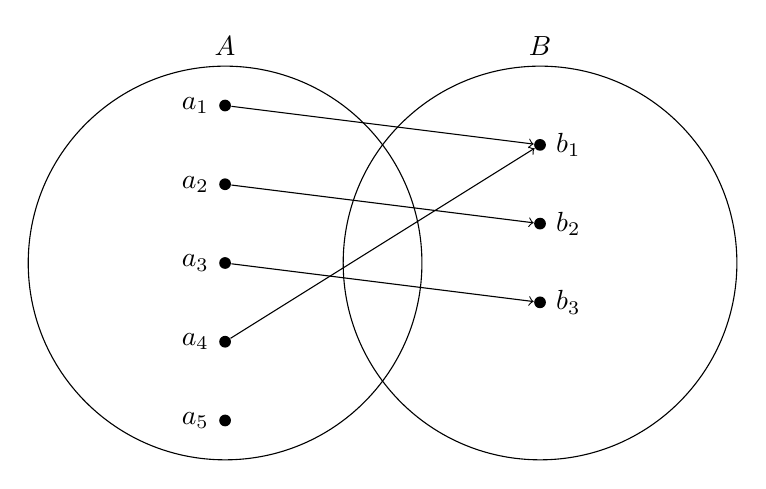
\begin{tikzpicture}
      % Conjuntos A e B
      \node[draw, circle, minimum width=3cm, minimum height=5cm, label=above:\( A \)] (A) at (0,0) {};
      \node[draw, circle, minimum width=3cm, minimum height=5cm, label=above:\( B \)] (B) at (4,0) {};

      % Elementos de A
      \node[fill, circle, inner sep=1.5pt, label=left:\( a_1 \)] (a1) at (0,2) {};
      \node[fill, circle, inner sep=1.5pt, label=left:\( a_2 \)] (a2) at (0,1) {};
      \node[fill, circle, inner sep=1.5pt, label=left:\( a_3 \)] (a3) at (0,0) {};
      \node[fill, circle, inner sep=1.5pt, label=left:\( a_4 \)] (a4) at (0,-1) {};
      \node[fill, circle, inner sep=1.5pt, label=left:\( a_5 \)] (a5) at (0,-2) {};

      % Elementos de B
      \node[fill, circle, inner sep=1.5pt, label=right:\( b_1 \)] (b1) at (4,1.5) {};
      \node[fill, circle, inner sep=1.5pt, label=right:\( b_2 \)] (b2) at (4,0.5) {};
      \node[fill, circle, inner sep=1.5pt, label=right:\( b_3 \)] (b3) at (4,-0.5) {};

      % Setas representando a relação funcional (ajuste conforme necessário)
      \draw[->] (a1) -- (b1);
      \draw[->] (a2) -- (b2);
      \draw[->] (a3) -- (b3);
      \draw[->] (a4) -- (b1);
      % Adicione mais setas se houver outras relações

    \end{tikzpicture}
  \end{center}
\end{frame}

\begin{frame}
  \frametitle{Funções - Exemplos}

  \begin{itemize}
    \item \( f : \mathbb{N}_0 \rightarrow \mathbb{N}_0 \) definida por \( f(x) = x^2 + 1 \)
    
    \item \( \text{abs} : \mathbb{Z} \rightarrow \mathbb{N}_0 \) definida por:
    \[
    \text{abs}(x) = 
    \begin{cases} 
      x & \text{se } x \geq 0 \\
      -x & \text{caso contrário}
    \end{cases}
    \]
    
    \item \( \text{distancia} : \mathbb{R}^2 \times \mathbb{R}^2 \rightarrow \mathbb{R} \) definida por:
    \[
    \text{distancia}((x_1, y_1),(x_2, y_2)) = \sqrt{(x_2 - x_1)^2 + (y_2 - y_1)^2}
    \]
  \end{itemize}

\end{frame}

\begin{frame}
  \frametitle{Função Parcial - Exemplo}

  \textbf{Definição (Função Parcial):}
  Uma função parcial \( f \) do conjunto \( A \) para o conjunto \( B \) (escrita como \( f : A \nrightarrow B \)) é dada por uma relação funcional \( G \) sobre \( A \) e \( B \). A relação \( G \) é chamada de gráfico de \( f \).

  \vspace{0.5cm}

  Escrevemos \( f(x) = y \) para \( (x, y) \in G \) e dizemos que \( y \) é a imagem de \( x \) sob \( f \). Se não existir \( y \in B \) com \( (x, y) \in G \), então \( f(x) \) é indefinido.

  Função parcial \( r : \mathbb{Z} \times \mathbb{Z} \nrightarrow \mathbb{Q} \) definida por:
  \[
  r(n, d) = 
  \begin{cases} 
    \frac{n}{d} & \text{se } d \neq 0 \\
    \text{indefinido} & \text{caso contrário}
  \end{cases}
  \]

  \begin{itemize}
    \item Esta função representa a divisão de dois números inteiros.
    \item A função é indefinida quando o denominador é zero, pois a divisão por zero não é permitida.
  \end{itemize}

\end{frame}

\begin{frame}
  \frametitle{Funções Parciais}


  \vspace{0.5cm}

  Função parcial \( r : \mathbb{Z} \times \mathbb{Z} \nrightarrow \mathbb{Q} \) definida por:
  \[
  r(n, d) = 
  \begin{cases} 
    \frac{n}{d} & \text{se } d \neq 0 \\
    \text{indefinido} & \text{caso contrário}
  \end{cases}
  \]
  possui gráfico \( \{((n, d), \frac{n}{d}) | n \in \mathbb{Z}, d \in \mathbb{Z} \setminus \{0\}\} \subseteq \mathbb{Z}^2 \times \mathbb{Q} \).

\end{frame}

\begin{frame}
  \frametitle{Domínio (de Definição), Codomínio e Imagem}

  \textbf{Definição (domínio de definição, codomínio, imagem):}
  Seja \( f : A \nrightarrow B \) uma função parcial.
  O conjunto \( A \) é chamado de domínio de \( f \) e o conjunto \( B \) é o seu codomínio.
  O domínio de definição de \( f \) é o conjunto
  \[
  \text{dom}(f) = \{x \in A | \exists y \in B \text{ tal que } f(x) = y\}.
  \]
  A imagem (ou conjunto imagem) de \( f \) é o conjunto
  \[
  \text{img}(f) = \{y | \exists x \in A \text{ tal que } f(x) = y\}.
  \]

  \begin{columns}
    \begin{column}{0.5\textwidth}
      \centering
      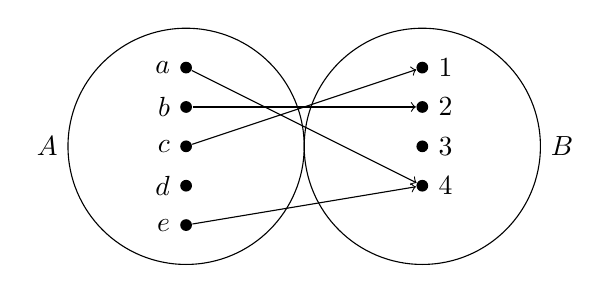
\begin{tikzpicture}
        % Conjuntos A e B
        \node[draw, circle, minimum size=3cm, label=left:\( A \)] (A) at (0,0) {};
        \node[draw, circle, minimum size=3cm, label=right:\( B \)] (B) at (3,0) {};

        % Elementos de A
        \foreach \value/\name in {1/a,0.5/b,0/c,-0.5/d,-1/e} {
          \node[fill, circle, inner sep=1.5pt, label=left:\( \name \)] (a\name) at (0,\value) {};
        }

        % Elementos de B
        \foreach \value/\name in {1/1,0.5/2,0/3,-0.5/4} {
          \node[fill, circle, inner sep=1.5pt, label=right:\( \name \)] (b\name) at (3,\value) {};
        }

        % Setas representando a função
        \draw[->] (aa) -- (b4);
        \draw[->] (ab) -- (b2);
        \draw[->] (ac) -- (b1);
        \draw[->] (ae) -- (b4);
      \end{tikzpicture}
    \end{column}

    \begin{column}{0.5\textwidth}
      \( f : \{a, b, c, d, e\} \nrightarrow \{1, 2, 3, 4\} \) \\
      \( f(a) = 4, f(b) = 2, f(c) = 1, f(e) = 4 \) \\
      domínio \( \{a, b, c, d, e\} \) \\
      codomínio \( \{1, 2, 3, 4\} \) \\
      domínio de definição \( \text{dom}(f) = \{a, b, c, e\} \) \\
      imagem \( \text{img}(f) = \{1, 2, 4\} \)
    \end{column}
  \end{columns}

\end{frame}
\begin{frame}
  \frametitle{Preimagem}

  A preimagem contém todos os elementos do domínio que são mapeados para elementos dados do contra-domínio.

  \textbf{Definição (Preimagem):}
  Seja \( f : A \nrightarrow B \) uma função parcial e \( Y \subseteq B \).
  A preimagem de \( Y \) sob \( f \) é o conjunto
  \[
  f^{-1}[Y] = \{x \in A | f(x) \in Y\}.
  \]

      \centering
      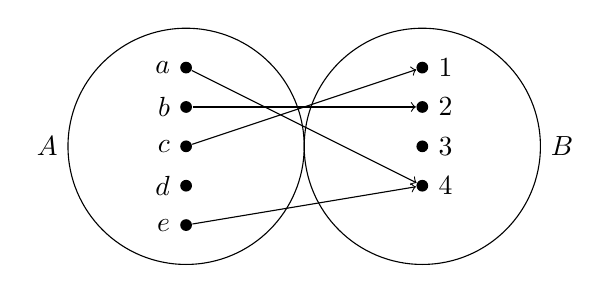
\begin{tikzpicture}
        % Conjuntos A e B
        \node[draw, circle, minimum size=3cm, label=left:\( A \)] (A) at (0,0) {};
        \node[draw, circle, minimum size=3cm, label=right:\( B \)] (B) at (3,0) {};

        % Elementos de A
        \foreach \value/\name in {1/a,0.5/b,0/c,-0.5/d,-1/e} {
          \node[fill, circle, inner sep=1.5pt, label=left:\( \name \)] (a\name) at (0,\value) {};
        }

        % Elementos de B
        \foreach \value/\name in {1/1,0.5/2,0/3,-0.5/4} {
          \node[fill, circle, inner sep=1.5pt, label=right:\( \name \)] (b\name) at (3,\value) {};
        }

        % Setas representando a função
        \draw[->] (aa) -- (b4);
        \draw[->] (ab) -- (b2);
        \draw[->] (ac) -- (b1);
        \draw[->] (ae) -- (b4);
      \end{tikzpicture}
    

\end{frame}

\begin{frame}
  \frametitle{Funções Totais}

  \textbf{Definição (Função Total):}
  Uma função (total) \( f : A \rightarrow B \) do conjunto \( A \) para o conjunto \( B \) é uma função parcial de \( A \) para \( B \) tal que \( f(x) \) é definido para todo \( x \in A \).
  \begin{itemize}
    \item Não há diferença entre o domínio e o domínio de definição.
  \end{itemize}

  \begin{center}
    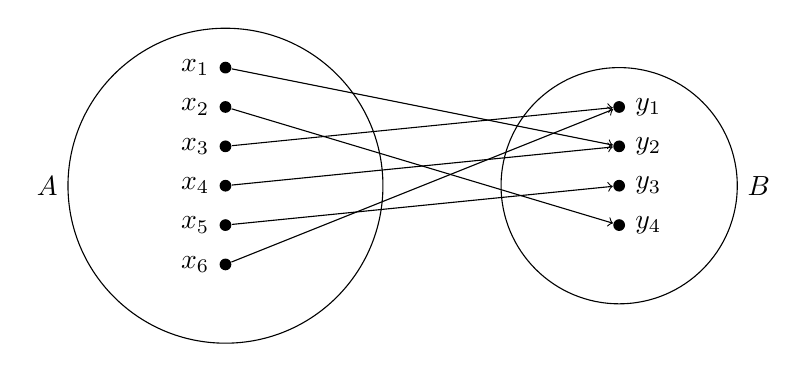
\begin{tikzpicture}
      % Conjuntos A e B
      \node[draw, circle, minimum size=4cm, label=left:\( A \)] (A) at (0,0) {};
      \node[draw, circle, minimum size=3cm, label=right:\( B \)] (B) at (5,0) {};

      % Elementos de A
      \node[fill, circle, inner sep=1.5pt, label=left:\( x_1 \)] (a1) at (0,1.5) {};
      \node[fill, circle, inner sep=1.5pt, label=left:\( x_2 \)] (a2) at (0,1) {};
      \node[fill, circle, inner sep=1.5pt, label=left:\( x_3 \)] (a3) at (0,0.5) {};
      \node[fill, circle, inner sep=1.5pt, label=left:\( x_4 \)] (a4) at (0,0) {};
      \node[fill, circle, inner sep=1.5pt, label=left:\( x_5 \)] (a5) at (0,-0.5) {};
      \node[fill, circle, inner sep=1.5pt, label=left:\( x_6 \)] (a6) at (0,-1) {};

      % Elementos de B
      \node[fill, circle, inner sep=1.5pt, label=right:\( y_1 \)] (b1) at (5,1) {};
      \node[fill, circle, inner sep=1.5pt, label=right:\( y_2 \)] (b2) at (5,0.5) {};
      \node[fill, circle, inner sep=1.5pt, label=right:\( y_3 \)] (b3) at (5,0) {};
      \node[fill, circle, inner sep=1.5pt, label=right:\( y_4 \)] (b4) at (5,-0.5) {};

      % Setas representando a função total
      \draw[->] (a1) -- (b2);
      \draw[->] (a2) -- (b4);
      \draw[->] (a3) -- (b1);
      \draw[->] (a4) -- (b2);
      \draw[->] (a5) -- (b3);
      \draw[->] (a6) -- (b1);
    \end{tikzpicture}
  \end{center}
\end{frame}

\begin{frame}
  \frametitle{Especificando uma Função}

  Algumas formas comuns de especificar uma função:
  \begin{itemize}
    \item Listando o mapeamento explicitamente, por exemplo:
    \[ f(a) = 4, \ f(b) = 2, \ f(c) = 1, \ f(e) = 4 \]
    ou
    \[ f = \{a \mapsto 4, \ b \mapsto 2, \ c \mapsto 1, \ e \mapsto 4\} \]
    
    \item Por uma fórmula, por exemplo:
    \[ f(x) = x^2 + 1 \]
    
    \item Por recorrência, por exemplo:
    \[ 0! = 1 \]
    e
    \[ n! = n(n - 1)! \ \text{para} \ n > 0 \]
    
    \item Em termos de outras funções, por exemplo: inversa, composição.
  \end{itemize}
\end{frame}

\begin{frame}[fragile]
  \frametitle{Relação com Funções em Programação}

  \begin{lstlisting}[language=Python, basicstyle=\ttfamily, keywordstyle=\color{blue}, commentstyle=\color{green}, stringstyle=\color{red}]
def factorial(n):
    if n == 0:
        return 1
    else:
        return n * factorial(n-1)
  \end{lstlisting}

  \begin{itemize}
    \item Relação entre recursão e recorrência.
  \end{itemize}
\end{frame}

\begin{frame}[fragile]
  \frametitle{Relação com Funções em Programação}

  \begin{lstlisting}[language=Python, basicstyle=\ttfamily, keywordstyle=\color{blue}, commentstyle=\color{green}, stringstyle=\color{red}]
def foo(n):
    value = ...
    while <some condition>:
        ...
        value = ...
    return value
  \end{lstlisting}

  \begin{itemize}
    \item Pode não terminar em todas as entradas.
    \item O valor é indefinido para tais entradas.
    \item Ciência da computação teórica: função parcial.
  \end{itemize}
\end{frame}

\begin{frame}[fragile]
  \frametitle{Relação com Funções em Programação}

  \begin{lstlisting}[language=Python, basicstyle=\ttfamily, keywordstyle=\color{blue}, commentstyle=\color{green}, stringstyle=\color{red}]
import random
counter = 0

def bar(n):
    print("Ola! Recebi a entrada", n)
    global counter
    counter += 1
    return random.choice([1,2,n])
  \end{lstlisting}

  \begin{itemize}
    \item Funções em programação nem sempre calculam funções matemáticas (exceto em linguagens puramente funcionais).
    \item Além disso, nem todas as funções matemáticas são computáveis.
  \end{itemize}
\end{frame}

\begin{frame}
  \frametitle{Operações em Funções Parciais}

\end{frame}

\begin{frame}
  \frametitle{Restrições e Extensões}

  \textbf{Definição (restrição e extensão):}
  \begin{itemize}
    \item Seja \( f: A \nrightarrow B \) uma função parcial e \( X \subseteq A \). A restrição de \( f \) a \( X \) é a função parcial \( f|_X: X \nrightarrow B \) tal que \( f|_X(x) = f(x) \) para todo \( x \in X \).

    \item Uma função \( f_0: A_0 \nrightarrow B \) é chamada de extensão de \( f \) se \( A \subseteq A_0 \) e \( f_0|_A = f \).

    \item A restrição de \( f \) ao seu domínio de definição é uma função total.
  \end{itemize}

\end{frame}

\begin{frame}
  \frametitle{Composição de Funções}

  \textbf{Definição (Composição de funções parciais):}
  Sejam \( f: A \nrightarrow B \) e \( g: B \nrightarrow C \) funções parciais.
  A composição de \( f \) e \( g \) é \( g \circ f: A \nrightarrow C \) definida por:
  \[
  (g \circ f)(x) = 
  \begin{cases} 
  g(f(x)) & \text{se } f \text{ é definida para } x \text{ e } g \text{ é definida para } f(x) \\
  \text{indefinido} & \text{caso contrário}
  \end{cases}
  \]

  \textbf{Observações:}
  \begin{itemize}
    \item Corresponde à composição de relações dos gráficos.
    \item Se \( f \) e \( g \) são funções, sua composição é uma função.
  \end{itemize}

  \textbf{Exemplo:}
  \begin{align*}
  f : \mathbb{N}_0 \rightarrow \mathbb{N}_0 & \text{ com } f(x) = x^2 \\
  g : \mathbb{N}_0 \rightarrow \mathbb{N}_0 & \text{ com } g(x) = x + 3 \\
  (g \circ f)(x) & = ?
  \end{align*}
\end{frame}

\begin{frame}
  \frametitle{Composição de Funções: \(g \circ f\)}
  
  Dadas as funções:
  \begin{align*}
    f(x) &= x^2 \\
    g(x) &= x + 3
  \end{align*}
  
  A composição \(g \circ f\) é:
  \[ (g \circ f)(x) = g(f(x)) \]
  
  Substituindo as expressões para \(f\) e \(g\), obtemos:
  \[ (g \circ f)(x) = x^2 + 3 \]
  
  Portanto, \((g \circ f)(x) = x^2 + 3\).
\end{frame}

\begin{frame}
  \frametitle{Propriedades da Composição de Funções}

  A composição de funções é:
  \begin{itemize}
    \item \textbf{Não comutativa}:
    \begin{align*}
      f : \mathbb{N}_0 &\to \mathbb{N}_0 \quad \text{com} \quad f(x) = x^2 \\
      g : \mathbb{N}_0 &\to \mathbb{N}_0 \quad \text{com} \quad g(x) = x + 3 \\
      (g \circ f)(x) &= x^2 + 3 \\
      (f \circ g)(x) &= (x + 3)^2
    \end{align*}
    
    \item \textbf{Associativa}, ou seja, \( h \circ (g \circ f) = (h \circ g) \circ f \)
    \begin{itemize}
      \item Análogo à associatividade da composição de relações.
    \end{itemize}
  \end{itemize}
\end{frame}

\begin{frame}
  \frametitle{Composição de Funções na Programação}

  
  Como fariamos composiçao de funcoes?
  
\end{frame}

\begin{frame}
  \frametitle{Propriedades das Funções}

  \begin{itemize}
    \item Funções parciais mapeiam cada elemento de seu domínio para no máximo um elemento de seu contradomínio, enquanto funções totais mapeiam para exatamente um valor.
    \item Elementos diferentes do domínio podem ter a mesma imagem.
    \item Pode haver valores no contradomínio que não são a imagem de nenhum elemento do domínio.
    \item Muitas vezes queremos excluir tais casos e definir propriedades adicionais para expressar isso rapidamente.
  \end{itemize}
\end{frame}



\begin{frame}
  \frametitle{Funções Injetivas}

  Uma função injetiva mapeia elementos distintos de seu domínio para elementos distintos de seu contradomínio.

  \textbf{Definição (Função Injetiva)}: \\
  Uma função \( f : A \rightarrow B \) é injetiva (também chamada de um-para-um ou injeção) se, para todos \( x, y \in A \) com \( x \neq y \), tem-se que \( f(x) \neq f(y) \).


\end{frame}

\begin{frame}{Funções Injetivas e Não Injetivas}

\begin{center}
    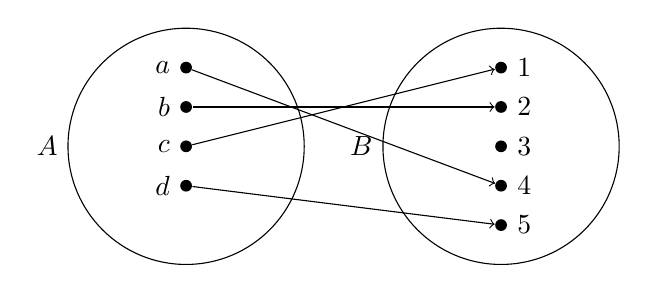
\begin{tikzpicture}
      % Conjuntos A e B
      \node[draw, circle, minimum size=3cm, label=left:\( A \)] (A) at (0,0) {};
      \node[draw, circle, minimum size=3cm, label=left:\( B \)] (B) at (4,0) {};

      % Elementos de A
      \node[fill, circle, inner sep=1.5pt, label=left:\( a \)] (a1) at (0,1) {};
      \node[fill, circle, inner sep=1.5pt, label=left:\( b \)] (a2) at (0,0.5) {};
      \node[fill, circle, inner sep=1.5pt, label=left:\( c \)] (a3) at (0,0) {};
      \node[fill, circle, inner sep=1.5pt, label=left:\( d \)] (a4) at (0,-0.5) {};

      % Elementos de B
      \node[fill, circle, inner sep=1.5pt, label=right:\( 1 \)] (b1) at (4,1) {};
      \node[fill, circle, inner sep=1.5pt, label=right:\( 2 \)] (b2) at (4,0.5) {};
      \node[fill, circle, inner sep=1.5pt, label=right:\( 3 \)] (b3) at (4,0) {};
      \node[fill, circle, inner sep=1.5pt, label=right:\( 4 \)] (b4) at (4,-0.5) {};
      \node[fill, circle, inner sep=1.5pt, label=right:\( 5 \)] (b5) at (4,-1) {};

      % Setas representando a função não injetiva
      \draw[->] (a1) -- (b4);
      \draw[->] (a2) -- (b2);
      \draw[->] (a3) -- (b1);
      \draw[->] (a4) -- (b5);
    \end{tikzpicture}
    
    \vspace{0.5cm}

    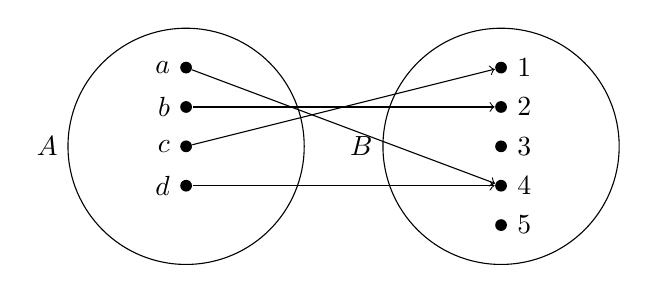
\begin{tikzpicture}
      % Conjuntos A e B
      \node[draw, circle, minimum size=3cm, label=left:\( A \)] (A) at (0,0) {};
      \node[draw, circle, minimum size=3cm, label=left:\( B \)] (B) at (4,0) {};

      % Elementos de A
      \node[fill, circle, inner sep=1.5pt, label=left:\( a \)] (a1) at (0,1) {};
      \node[fill, circle, inner sep=1.5pt, label=left:\( b \)] (a2) at (0,0.5) {};
      \node[fill, circle, inner sep=1.5pt, label=left:\( c \)] (a3) at (0,0) {};
      \node[fill, circle, inner sep=1.5pt, label=left:\( d \)] (a4) at (0,-0.5) {};

      % Elementos de B
      \node[fill, circle, inner sep=1.5pt, label=right:\( 1 \)] (b1) at (4,1) {};
      \node[fill, circle, inner sep=1.5pt, label=right:\( 2 \)] (b2) at (4,0.5) {};
      \node[fill, circle, inner sep=1.5pt, label=right:\( 3 \)] (b3) at (4,0) {};
      \node[fill, circle, inner sep=1.5pt, label=right:\( 4 \)] (b4) at (4,-0.5) {};
      \node[fill, circle, inner sep=1.5pt, label=right:\( 5 \)] (b5) at (4,-1) {};

      % Setas representando a função não injetiva
      \draw[->] (a1) -- (b4);
      \draw[->] (a2) -- (b2);
      \draw[->] (a3) -- (b1);
      \draw[->] (a4) -- (b4);
    \end{tikzpicture}
\end{center}
\end{frame}



\begin{frame}{Funções Injetivas – Exemplos}

  Quais destas funções são injetivas?
  
  \begin{itemize}
      \item \( f : \mathbb{Z} \rightarrow \mathbb{N}_0 \) com \( f(x) = |x| \)
      \item \( g : \mathbb{N}_0 \rightarrow \mathbb{N}_0 \) com \( g(x) = x^2 \)
      \item \( h : \mathbb{N}_0 \rightarrow \mathbb{N}_0 \) definida por 
      \[
      h(x) = 
      \begin{cases} 
        x - 1 & \text{se } x \text{ é ímpar} \\
        x + 1 & \text{se } x \text{ é par} 
      \end{cases}
      \]
  \end{itemize}
  
  \end{frame}


\begin{frame}{Composição de Funções Injetivas}

  \textbf{Teorema:} \\
  Se \( f : A \rightarrow B \) e \( g : B \rightarrow C \) são funções injetivas, então \( g \circ f \) também é injetiva.
  
  \textbf{Prova:} \\
  Considere elementos arbitrários \( x, y \in A \) com \( x \neq y \). \\
  Como \( f \) é injetiva, sabemos que \( f(x) \neq f(y) \). \\
  Como \( g \) é injetiva, isso implica que \( g(f(x)) \neq g(f(y)) \). \\
  Com a definição de \( g \circ f \), concluímos que \\
  \( (g \circ f)(x) \neq (g \circ f)(y) \). \\
  Portanto, isso mostra que \( g \circ f \) é injetiva.
  
  \end{frame}
  

\begin{frame}{Funções Sobrejetivas}

  \textbf{Definição:} \\
  Uma função é dita sobrejetiva se, e somente se, para todo elemento \( y \) do conjunto codomínio, existe pelo menos um elemento \( x \) no domínio tal que \( f(x) = y \).
  
  Em outras palavras, uma função \( f : A \rightarrow B \) é sobrejetiva (também chamada de "sobre" ou "sobrejeção") se sua imagem é igual ao seu codomínio.
  
  \end{frame}


\begin{frame}{Funções Sobrejetivas e Não Sobrejetivas}

  \begin{center}
      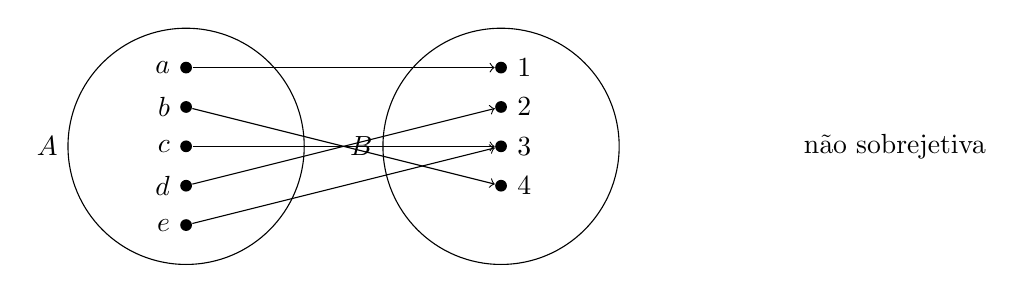
\begin{tikzpicture}[node distance=3cm, auto]
        % Conjuntos A e B
        \node[draw, circle, minimum size=3cm, label=left:\( A \)] (A) at (0,0) {};
        \node[draw, circle, minimum size=3cm, label=left:\( B \)] (B) at (4,0) {};
  
        % Elementos de A
        \node[fill, circle, inner sep=1.5pt, label=left:\( a \)] (a1) at (0,1) {};
        \node[fill, circle, inner sep=1.5pt, label=left:\( b \)] (a2) at (0,0.5) {};
        \node[fill, circle, inner sep=1.5pt, label=left:\( c \)] (a3) at (0,0) {};
        \node[fill, circle, inner sep=1.5pt, label=left:\( d \)] (a4) at (0,-0.5) {};
        \node[fill, circle, inner sep=1.5pt, label=left:\( e \)] (a5) at (0,-1) {};
  
        % Elementos de B
        \node[fill, circle, inner sep=1.5pt, label=right:\( 1 \)] (b1) at (4,1) {};
        \node[fill, circle, inner sep=1.5pt, label=right:\( 2 \)] (b2) at (4,0.5) {};
        \node[fill, circle, inner sep=1.5pt, label=right:\( 3 \)] (b3) at (4,0) {};
        \node[fill, circle, inner sep=1.5pt, label=right:\( 4 \)] (b4) at (4,-0.5) {};
  
        % Setas representando a função não sobrejetiva
        \draw[->] (a1) -- (b1);
        \draw[->] (a2) -- (b4);
        \draw[->] (a3) -- (b3);
        \draw[->] (a4) -- (b2);
        \draw[->] (a5) -- (b3);
  
        % Label para função não sobrejetiva
        \node [right of=B, node distance=5cm] (label1) {não sobrejetiva};
      \end{tikzpicture}
  
      \vspace{0.5cm}
  
      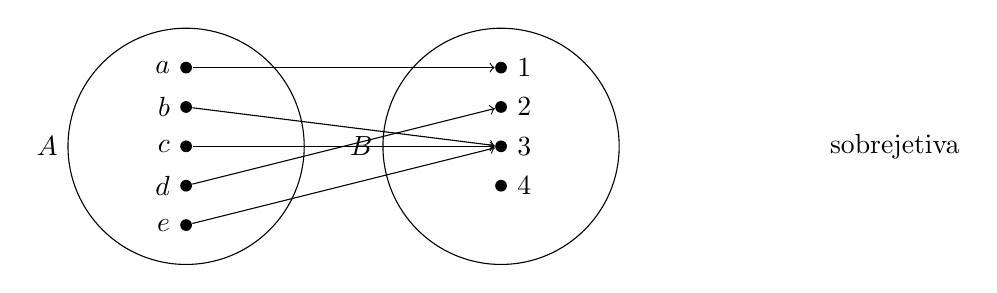
\begin{tikzpicture}[node distance=3cm, auto]
        % Conjuntos A e B
        \node[draw, circle, minimum size=3cm, label=left:\( A \)] (A) at (0,0) {};
        \node[draw, circle, minimum size=3cm, label=left:\( B \)] (B) at (4,0) {};
        
        % Elementos de A
        \node[fill, circle, inner sep=1.5pt, label=left:\( a \)] (a1) at (0,1) {};
        \node[fill, circle, inner sep=1.5pt, label=left:\( b \)] (a2) at (0,0.5) {};
        \node[fill, circle, inner sep=1.5pt, label=left:\( c \)] (a3) at (0,0) {};
        \node[fill, circle, inner sep=1.5pt, label=left:\( d \)] (a4) at (0,-0.5) {};
        \node[fill, circle, inner sep=1.5pt, label=left:\( e \)] (a5) at (0,-1) {};
  
        % Elementos de B
        \node[fill, circle, inner sep=1.5pt, label=right:\( 1 \)] (b1) at (4,1) {};
        \node[fill, circle, inner sep=1.5pt, label=right:\( 2 \)] (b2) at (4,0.5) {};
        \node[fill, circle, inner sep=1.5pt, label=right:\( 3 \)] (b3) at (4,0) {};
        \node[fill, circle, inner sep=1.5pt, label=right:\( 4 \)] (b4) at (4,-0.5) {};
  
        % Setas representando a função sobrejetiva
        \draw[->] (a1) -- (b1);
        \draw[->] (a2) -- (b3);
        \draw[->] (a3) -- (b3);
        \draw[->] (a4) -- (b2);
        \draw[->] (a5) -- (b3);
  
        % Label para função sobrejetiva
        \node [right of=B, node distance=5cm] (label2) {sobrejetiva};
      \end{tikzpicture}
  \end{center}
  \end{frame}
  
  \begin{frame}{Funções Sobrejetivas – Exemplos}
    Quais destas funções são sobrejetivas?
    \begin{enumerate}
      \item $f : \mathbb{Z} \rightarrow \mathbb{N}_0$ com $f(x) = |x|$
      \item $g : \mathbb{N}_0 \rightarrow \mathbb{N}_0$ com $g(x) = x^2$
      \item $h : \mathbb{N}_0 \rightarrow \mathbb{N}_0$ com
      \[
      h(x) = \begin{cases}
        x - 1 & \text{se $x$ é ímpar} \\
        x + 1 & \text{se $x$ é par}
      \end{cases}
      \]
    \end{enumerate}
  \end{frame}

  \begin{frame}{Funções Bijectivas}
    Uma função bijectiva emparelha cada elemento do seu domínio com exatamente um elemento do seu contradomínio, e cada elemento do contradomínio é emparelhado com exatamente um elemento do domínio.
  
    \textbf{Definição (Função Bijectiva)}
    Uma função é bijectiva (também chamada de correspondência um a um ou bijeção) se ela for injetiva e sobrejetiva.
  
    \begin{center}
      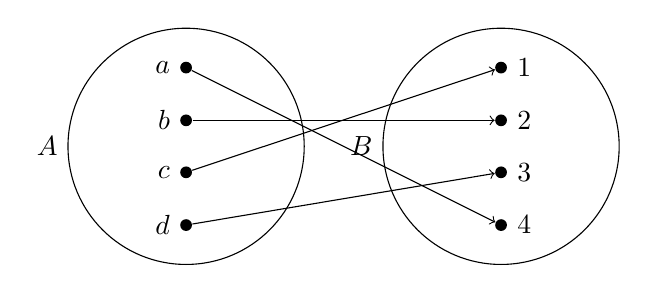
\begin{tikzpicture}
        % Conjuntos A e B
        \node[draw, circle, minimum size=3cm, label=left:\( A \)] (A) at (0,0) {};
        \node[draw, circle, minimum size=3cm, label=left:\( B \)] (B) at (4,0) {};
  
        % Elementos de A
        \node[fill, circle, inner sep=1.5pt, label=left:\( a \)] (a1) at (0,1) {};
        \node[fill, circle, inner sep=1.5pt, label=left:\( b \)] (a2) at (0,0.33) {};
        \node[fill, circle, inner sep=1.5pt, label=left:\( c \)] (a3) at (0,-0.33) {};
        \node[fill, circle, inner sep=1.5pt, label=left:\( d \)] (a4) at (0,-1) {};
  
        % Elementos de B
        \node[fill, circle, inner sep=1.5pt, label=right:\( 1 \)] (b1) at (4,1) {};
        \node[fill, circle, inner sep=1.5pt, label=right:\( 2 \)] (b2) at (4,0.33) {};
        \node[fill, circle, inner sep=1.5pt, label=right:\( 3 \)] (b3) at (4,-0.33) {};
        \node[fill, circle, inner sep=1.5pt, label=right:\( 4 \)] (b4) at (4,-1) {};
  
        % Setas representando a bijeção
        \draw[->] (a1) -- (b4);
        \draw[->] (a2) -- (b2);
        \draw[->] (a3) -- (b1);
        \draw[->] (a4) -- (b3);
      \end{tikzpicture}
    \end{center}
  
    \textbf{Corolário}
    A composição de duas funções bijetivas também é bijetiva.
  \end{frame}
  
  \begin{frame}{Funções Bijectivas - Exemplos}
    Quais dessas funções são bijetivas?
    
    \textbf{I.} \(f : \mathbb{Z} \to \mathbb{N}_0\) com \(f (x) = |x|\)
  
    \textbf{II.} \(g : \mathbb{N}_0 \to \mathbb{N}_0\) com \(g(x) = x^2\)
  
    \textbf{III.} \(h : \mathbb{N}_0 \to \mathbb{N}_0\) com
    \[
      h(x) =
      \begin{cases}
        x - 1 & \text{se } x \text{ é ímpar} \\
        x + 1 & \text{se } x \text{ é par}
      \end{cases}
    \]
    
  
  \end{frame}

  \begin{frame}{Funções Bijectivas - Exemplos}
    Quais dessas funções são bijetivas?
    
    \textbf{I.} \(f : \mathbb{Z} \to \mathbb{N}_0\) com \(f (x) = |x|\)
  
    \textbf{II.} \(g : \mathbb{N}_0 \to \mathbb{N}_0\) com \(g(x) = x^2\)
  
    \textbf{III.} \(h : \mathbb{N}_0 \to \mathbb{N}_0\) com
    \[
      h(x) =
      \begin{cases}
        x - 1 & \text{se } x \text{ é ímpar} \\
        x + 1 & \text{se } x \text{ é par}
      \end{cases}
    \]
    
    \textbf{Resposta:}
    
    (I) A função \(f\) não é bijetiva, pois ela mapeia números negativos para zero e números positivos para valores positivos, então não cobre todo o contradomínio \(\mathbb{N}_0\).
  
    (II) A função \(g\) não é bijetiva, pois mapeia todos os números naturais para valores positivos, mas não cobre o zero.
  
    (III) A função \(h\) é bijetiva, pois ela mapeia cada número natural para outro número natural, e cada número natural é coberto.
  
  \end{frame}

  \begin{frame}{Função Inversa}
    \textbf{Definição:}
    
    Seja \(f : A \to B\) uma bijeção.
    
    A função inversa de \(f\) é a função \(f^{-1} : B \to A\) tal que:
    
    \[f^{-1}(y) = x \quad \text{se e somente se} \quad f(x) = y.\]
    
    Ou seja, \(f^{-1}(y)\) é o elemento em \(A\) que mapeia para \(y\) sob a função \(f\).
  \end{frame}
  
  
  \begin{frame}{Função Inversa}

    \centering
    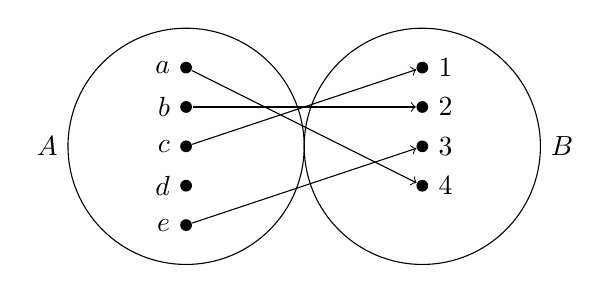
\begin{tikzpicture}
      % Conjuntos A e B
      \node[draw, circle, minimum size=3cm, label=left:\( A \)] (A) at (0,0) {};
      \node[draw, circle, minimum size=3cm, label=right:\( B \)] (B) at (3,0) {};
  
      % Elementos de A
      \foreach \value/\name in {1/a,0.5/b,0/c,-0.5/d,-1/e} {
        \node[fill, circle, inner sep=1.5pt, label=left:\( \name \)] (a\name) at (0,\value) {};
      }
  
      % Elementos de B
      \foreach \value/\name in {1/1,0.5/2,0/3,-0.5/4} {
        \node[fill, circle, inner sep=1.5pt, label=right:\( \name \)] (b\name) at (3,\value) {};
      }
  
      % Setas representando a função
      \draw[->] (aa) -- (b4);
      \draw[->] (ab) -- (b2);
      \draw[->] (ac) -- (b1);
      \draw[->] (ae) -- (b3);
    \end{tikzpicture}

    \centering
    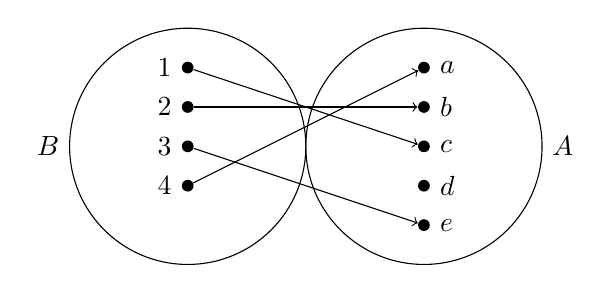
\begin{tikzpicture}
      % Conjuntos A e B
      \node[draw, circle, minimum size=3cm, label=left:\( B \)] (B) at (0,0) {};
      \node[draw, circle, minimum size=3cm, label=right:\( A \)] (A) at (3,0) {};
  
      % Elementos de A
      \foreach \value/\name in {1/a,0.5/b,0/c,-0.5/d,-1/e} {
        \node[fill, circle, inner sep=1.5pt, label=right:\( \name \)] (a\name) at (3,\value) {};
      }
  
      % Elementos de B
      \foreach \value/\name in {1/1,0.5/2,0/3,-0.5/4} {
        \node[fill, circle, inner sep=1.5pt, label=left:\( \name \)] (b\name) at (0,\value) {};
      }
  
      % Setas representando a função
      \draw[->] (b4) -- (aa);
      \draw[->] (b2) -- (ab);
      \draw[->] (b1) -- (ac);
      \draw[->] (b3) -- (ae);
    \end{tikzpicture}

  \end{frame}
  
  \begin{frame}{Função Inversa e Composição}
    \textbf{Teorema:}
    
    Seja \(f : A \to B\) uma bijeção.
    
    \begin{enumerate}
      \item Para todo \(x \in A\), temos \(f^{-1}(f(x)) = x\).
      \item Para todo \(y \in B\), temos \(f(f^{-1}(y)) = y\).
      \item \((f^{-1})^{-1} = f\).
    \end{enumerate}
    
    \textbf{Esboço da Prova:}
    
    \begin{enumerate}
      \item Para \(x \in A\), seja \(y = f(x)\). Então, \(f^{-1}(f(x)) = f^{-1}(y) = x\).
      \item Para \(y \in B\), existe exatamente um \(x\) tal que \(y = f(x)\). Com esse \(x\), temos \(f(f^{-1}(y)) = f(x) = y\).
      \item Pela definição de inversa, \((f^{-1})^{-1}(x) = y\) se e somente se \(f^{-1}(y) = x\) se e somente se \(f(x) = y\).
    \end{enumerate}
  \end{frame}
  
  \begin{frame}{Função Inversa e Composição}
    \textbf{Teorema:}
    
    Seja \(f : A \to B\) e \(g : B \to C\) bijeções.
    
    Então, \((g \circ f)^{-1} = f^{-1} \circ g^{-1}\).
    
    \textbf{Prova:}
    \begin{itemize}
    \item Precisamos mostrar que, para todo \(x \in C\), temos \((g \circ f)^{-1}(x) = (f^{-1} \circ g^{-1})(x)\).
    
    \item Considere um \(x \in C\) arbitrário e considere \(y = (g \circ f)^{-1}(x)\).
    
    \item Pela definição da inversa, \((g \circ f)(y) = x\).
    
    \item Seja \(z = f(y)\). Com \((g \circ f)(y) = g(f(y))\), sabemos que \(x = g(z)\).
    
    \item A partir de \(z = f(y)\), obtemos \(f^{-1}(z) = y\).
    
    \item A partir de \(x = g(z)\), obtemos \(g^{-1}(x) = z\).
    
    \item Isso nos dá \((f^{-1} \circ g^{-1})(x) = f^{-1}(g^{-1}(x)) = f^{-1}(z) = y\).
    \end{itemize}

  \end{frame}
  
  \begin{frame}{Resumo}
    \textbf{Função Injetiva:} Mapeia elementos distintos do seu domínio para elementos distintos do seu contradomínio.
  
    \textbf{Função Sobrejetiva:} Mapeia pelo menos um elemento para cada elemento do seu contradomínio.
  
    \textbf{Função Bijetiva:} É tanto injetiva quanto sobrejetiva, estabelecendo uma correspondência um a um.
  
    \textbf{Funções Bijetivas são Invertíveis:} A função inversa de $f$ mapeia a imagem de $x$ sob $f$ de volta a $x$.
  \end{frame}

  \begin{frame}{Funções sobre Conjuntos - Resumo}
    \textbf{Funções sobre Conjuntos na Programação:}
    
    \begin{itemize}
      \item Funções são mapeamentos de um conjunto de entrada para um conjunto de saída.
      \item Permitem modelar relações entre elementos de conjuntos.
      \item São amplamente utilizadas para resolver problemas matemáticos e lógicos na programação.
      \item Facilitam a abstração e a modularização do código.
    \end{itemize}
  \end{frame}
  
  \begin{frame}{Funções sobre Conjuntos na Programação - Análise}
    \textbf{Quando a Utilização de Funções sobre Conjuntos é Interessante?}
    
    \begin{itemize}
      \item \textbf{Modelagem Matemática:} Funções são ideais para representar relações matemáticas e cálculos.
      
      \item \textbf{Solução de Problemas Complexos:} São usadas para resolver problemas que envolvem conjuntos de dados complexos.
      
      \item \textbf{Manipulação de Dados:} Facilitam a manipulação, transformação e processamento de conjuntos de dados.
      
      \item \textbf{Abstração e Modularização:} Permitem dividir problemas complexos em funções menores e mais gerenciáveis.
      
      \item \textbf{Reutilização de Código:} Funções podem ser reaproveitadas em diferentes partes de um programa.
    \end{itemize}
  \end{frame}
    